\chapter{Trigonometry}

In the first half of this chapter the three trigonometric functions (sine, cosine and tangent) will be viewed as functions of angles. The second half of the chapter will approach trigonometry as functions of real numbers.
%---------------------------------------------------
% pythagorean theorem
%---------------------------------------------------
\section*{Pythagoras}
Pythagoras is one of the most well known historical figures in mathematics and philosophy, primarily for the his eponymous theorem. Given a right-angled triangle, the hypotenuse squared equals the sum of the squares of the other sides.
\begin{tcolorbox}[colback=white]
	\begin{multicols}{2}
		\begin{center}
			The Pythagorean Theorem:\\
			
			\vspace{1cm}$a^2+b^2=c^2$
		\end{center}
\columnbreak
\begin{center}
	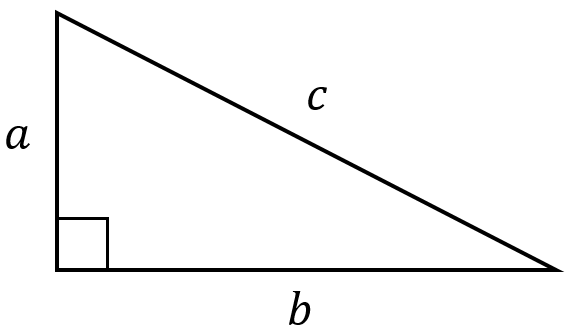
\includegraphics[width=6cm]{trigPythagoras}
\end{center}
	\end{multicols}
\end{tcolorbox}
This diagram will be the basis for a lot of our study of triangles. We will return to the Pythagorean theorem in section~\ref{sec:identities} when discussing some special trigonometry relationships.
%---------------------------------------------------
% the unit circle and radians
%---------------------------------------------------
\section{The Unit Circle}
It should come as no surprise that the convention for measuring angles should be the same as for measuring
the distance around the perimeter of the unit circle.. An angle is measured in degrees and is the amount of
rotation between two rays about a vertex. If the vertex is placed at the point $\left (0 ,0\right )$ and one ray is placed along the positive $x$-axis then we let the second ray go through the point $P (x ,y)$ on the unit circle so that the relationship between the angle and the arc length $t$ can be established. The convention is that the positive direction for measuring
angles is anticlockwise and the negative direction for measuring angles is clockwise. You will be aware that one complete cycle measures \ang{360}. One degree therefore is $\frac{1}{360}$\ of one complete cycle. In this subject the word revolution is often used instead of cycle. Other terms with which you might be familiar are ``a quarter turn" for \ang{90} and ``a half turn" for \ang{180}. 

If you draw a unit circle (centre $\left (0 ,0\right )$ radius $1$) then you can draw the ray through any terminal point and show the relationship between $t$ and the angle at the vertex $\left (0 ,0\right )$. 

Definition: If the unit circle is drawn and the distance $t$ is measured around the perimeter from $\left (1 ,0\right )$ to the point $P (x ,y)$ then we say the angle is measured as $t$ \emph{radians}. 

The abbreviation for radians is \textit{rad}. This abbreviation will be used in the examples.
Some books uses the term ``angles in standard position" to describe this situation. We
will not define this term unless it is unavoidable and will stick to rad.

\columnsep =30pt
\begin {multicols}{2}
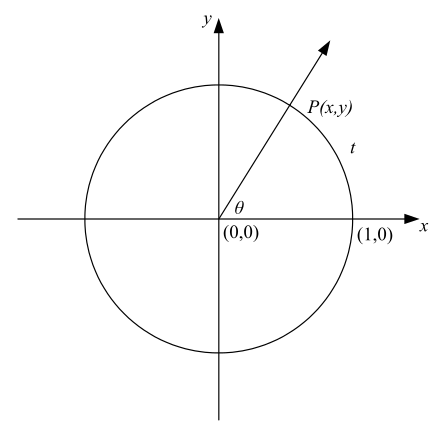
\includegraphics[width=6cm]{L4SZ281A}
\columnbreak

Using the language of geometry, the unit circle is cut by two rays one through the points $\left (0 ,0\right )$ and $\left (1 ,0\right )$ and the other through the points $\left (0 ,0\right )$ and $P \left (x ,y\right )$. 

$t$ is referred to as "the length of the arc". The angle $\theta $ between the two rays is referred to as "the angle \emph{subtended} at the point $\left (0 ,0\right )$". We will often leave out the word "subtended" however as it is implied. 
\end {multicols}
We can say therefore that the angle measured in radians is related to the same angle measured in degrees. the relationship between these two measures must be understood and must be able to be derived. 

\subsection*{Relationship between Degrees and Radians}
One complete revolution is \ang{360} if the angle is measured in degrees and $2 \pi $ if the angle is measured in radians. So
\begin{align*}2 \pi \text{}\mbox{rad} &  =  \ang{360} \\
\text{or\  \ }\pi \text{}\mbox{rad} &  =  \ang{180}
\end{align*}
You should derive this formula whenever you are asked to convert degrees to radians or radians
to degrees. 

\textbf{Example}
(a) Convert \ang{36} to radians 
(b) Convert $\frac{\pi }{3}$ $\mbox{rad}$ to degrees 
(c) Convert $1$ $\mbox{rad}$ to degrees 

\textbf{Solution}\begin{tasks}[before-skip = {0ex} , after-skip={-5ex}](3)
\task \begin{align*}\ang{180}  &  =  \pi \text{}\mbox{rad} \\
\ang{1}  &  =  \frac{\pi }{180}\text{}\mbox{rad} \\
\ang{36}  &  =  \frac{\pi }{180} \times 36 =\frac{\pi }{5}\text{}\mbox{rad}\end{align*}
\task
\begin{align*}\pi  \mbox{rad} &  =  \ang{180}  \\
\frac{\pi }{3} \mbox{rad} &  = \frac{\ang{180} }{3} =\ang{60} \end{align*}
\task
\begin{align*}\pi  \mbox{rad} &  =  \ang{180} \\
1 \mbox{rad} &  =  \frac{\ang{180} }{\pi } \\
 &  \approx   \ang{57.29577951}  \\
 &  \approx   \ang{57.3} \end{align*}
\end{tasks}
Note the similarity between the answers to (b) and (c). This is because $\frac{\pi }{3} =1.047197551$ so you would expect the values in degrees to be similar.  With this terminology we leave out the word measured when we talk about measuring angles. We say ``the angle is $\ang{60} $" when we mean it has been measured as $\ang{60} $ or ``the angle is $\frac{\pi }{3}$" to mean it has been measured as $\frac{\pi }{3}$ $\mbox{rad}$. Notice we always put in the degree symbol and often omit the units when the angle is measured in radians. Should units be omitted assume the angle is measured in radians. We often use the Greek symbol $\theta $\ for the angle subtended at the centre of the unit circle so $\theta  =\ang{60} $ or $\theta  =\frac{\pi }{3}$ are further examples of terminology that is commonly used.

\subsection*{Arc Length}
Let $\theta $ be the angle subtended at the centre for the ends of an arc of any circle then the fraction of the circumference of the circle is $\frac{\theta }{2 \pi }$ if $\theta $ is measured in radians and $\frac{\theta }{\ang{360}}$ if $\theta $ is measured in degrees. 

The length of the circumference of any circle whose radius is $r$ is $2 \pi  r$. If $\theta $ is measured in radians
\begin{equation*}\text{Length of arc} =\frac{\theta }{2 \pi } \times 2 \pi  r =\theta  r\text{or}r \theta 
\end{equation*}

If $\theta $ is measured in degrees
\begin{equation*}\text{Length of arc} =\frac{\theta }{\ang{360}} \times 2 \pi  r
\end{equation*}

The simplicity of the first formula shows why working with radians is preferred. 

\textbf{Example} Find the length of an arc that subtends an angle of \ang{45} at the centre of a circle whose radius is 9 cm. 

\textbf{Solution} \begin{tasks}[counter-format=(tsk[1]),before-skip = {0ex},after-skip={-5ex}](2)
	\task Method 1:\begin{eqnarray*}\text{Length of arc} &  = & \frac{\theta }{360 \mbox{{\ensuremath{{}^\circ}}}} \times 2 \pi  r \\
	&  = & \frac{45}{360} \times 2 \pi  \times 9 \\
	&  = & 2.25 \pi \text{}\mbox{cm} \\
	&  \approx  & 7.07\text{}\mbox{cm}\end{eqnarray*}
If an exact answer is required you should\\ leave the answer as $2.25 \pi $ $\mbox{cm}$. (Or $\frac{9 \pi }{4}$ $\mbox{cm}\text{.}$) 

\task Method 2: Change degrees to radians first
\begin{eqnarray*}180 \mbox{{\ensuremath{{}^\circ}}} &  = & \pi \text{}\mbox{rad} \\
	1 \mbox{{\ensuremath{{}^\circ}}} &  = & \frac{\pi }{180} \\
	45 \mbox{{\ensuremath{{}^\circ}}} &  = & \frac{\pi }{180} \times 45 \\
	&  = & \frac{\pi }{4}\end{eqnarray*}
Now, the length of arc $= r \theta = 9 \times \frac{\pi }{4} =\frac{9 \pi }{4}\text{}\mbox{cm}$.
\end{tasks}
%---------------------------------------------------
% Right-Angled Triangles: trig ratios
%---------------------------------------------------
\section{Right-Angled Triangles}
A right angled triangle is uniquely defined, if as well as the \ang{90} angle, you are given one side and one angle or two sides. To be given two angles does is not enough information as the scale of the triangle is not known. The sides of the triangle have names with respect to the angle of interest, $\theta$ in the diagram. 
\begin{multicols}{2}
\begin{center}
	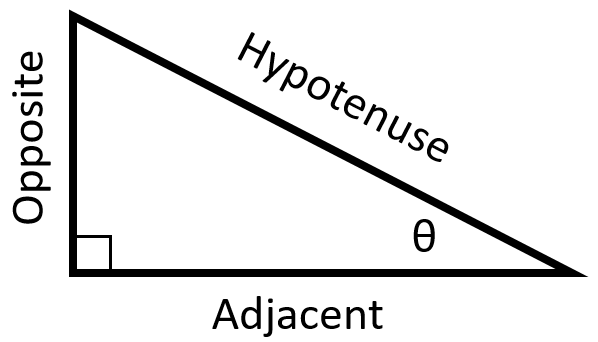
\includegraphics[width=7cm]{rightTriangle}
\end{center}
\columnbreak
Notice that if $\theta$ changes, then the sides opposite and adjacent are reversed. These side names are helpful in defining the trigonometric ratios of sine, cosine and tangent. The phrase \textbf{SOH-CAH-TOA} is useful to remember the ratios.
\end{multicols}


\begin{tcolorbox}
\begin{equation*}\text{sine }  \theta  =\frac{\text{opposite}}{\text{hypotenuse}}\text{;}\qquad\text{cosine }  \theta  =\frac{\text{adjacent}}{\text{hypotenuse}}\text{;}\qquad\text{tangent }  \theta  =\frac{\text{opposite}}{\text{adjacent}}
\end{equation*}\medskip
\hspace{2.5cm}S O H\hspace{3cm}C A H\hspace{4cm}T O A
\end{tcolorbox}

%----------------------------------------------------
\begin{multicols}{2}
	\textbf{Example 1} Find the unknown side $x$\\
	\begin{center}
		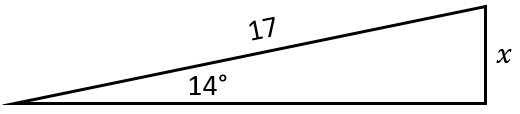
\includegraphics[width=8cm]{trigSide1}
	\end{center}

	\columnbreak
\textbf{Solution} Write the sine ratio and solve for $x$.\\
\begin{align*}\sin 14 &= \frac{x}{17}\\
x&=17\sin 14\\
x&=4.11\end{align*}
\end{multicols}

\begin{multicols}{2}
\textbf{Example 2} Find the unknown side $x$\\
\begin{center}
	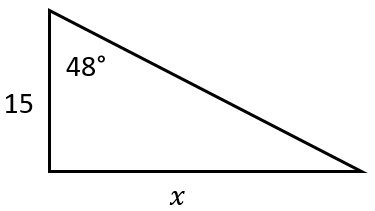
\includegraphics[width=6cm]{trigSide2}
\end{center}
	\columnbreak
\textbf{Solution} Write the tangent ratio and solve for $x$.
\begin{align*}\tan 48 = \frac{x}{15}\\
x=15\tan 28\\
x=16.7\end{align*}
\end{multicols}

The calculator gives approximate values of the trigonometric ratios. You must look at your question to check whether angles are in degrees or radians and ensure the calculator is first set in the right mode. Questions where degrees are to be used will give angles marked with a $^\circ$ symbol. 


When solving for an angle on your calculator you select the appropriate trigonometry ratio and use the \emph{shift} button with sin, cos or tan to find $\sin ^{ -1}$, $\cos ^{ -1}$ or $\tan ^{ -1}$. 
%----------------------------------------------------
\begin{multicols}{2}
	\textbf{Example 3} Find the unknown angle $x$\\
	\begin{center}
		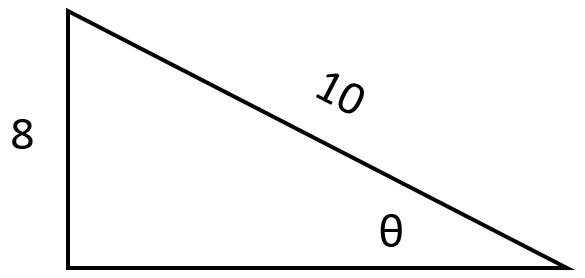
\includegraphics[width=7cm]{trigAngle1}
	\end{center}
	
	\columnbreak
	\textbf{Solution} Write the sine ratio and solve for $\theta$.\\
	\begin{align*}\sin \theta &= \frac{8}{10}\\
	\sin\theta&=0.8\\
	\theta&=\sin^{-1}(0.8)\\
	\theta&=\ang{53.1}
	\end{align*}
\end{multicols}

\begin{multicols}{2}
	\textbf{Example 4} Find the unknown angle $x$\\
	\begin{center}
		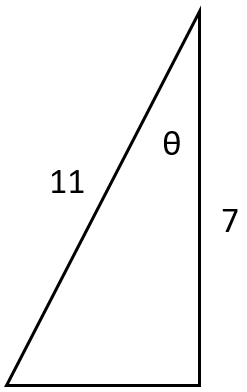
\includegraphics[width=4cm]{trigAngle2}
	\end{center}
	\columnbreak
	\textbf{Solution} Write the cosine ratio and solve for $\theta$.
	\begin{align*}\cos \theta = \frac{7}{11}\\
	\theta=\cos^{-1} \left(\frac{7}{11}\right)\\
	\theta=\ang{50.5}
	\end{align*}
\end{multicols}

%----------------------------------------------------
\textbf{Example 5}
The height of a steep cliff is to be measured from a point on the opposite side of the river. The following diagram shows the measurements taken. Estimate the height of the cliff.

\begin {multicols}{2}
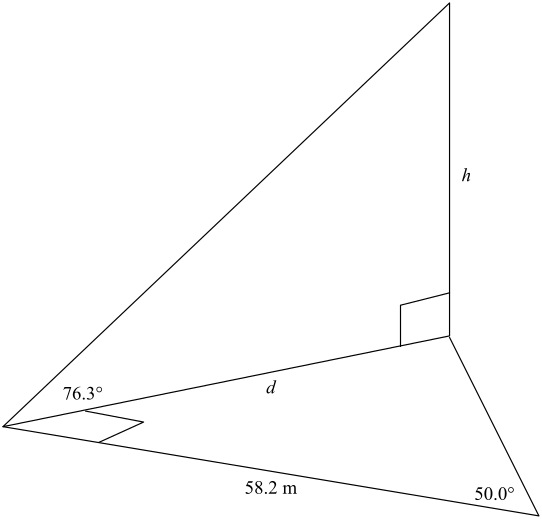
\includegraphics[width=8cm]{L4SZ281H}
\columnbreak
\begin{align*}\frac{d}{58.2} &  =  \tan  \ang{50.0}  \\
d &  =  58.2 \times \tan  \ang{50.0}  \\
\frac{h}{d} &  =  \tan  \ang{76.3}  \\
h &  =  d \times \tan  \ang{76.3}  \\
 &  =  58.2 \times \tan  \ang{50.0}  \times \tan  \ang{76.3}  \\
 &  \approx   284.526397 \\
 &  \approx   284.5 \mbox{m}\end{align*}
\end {multicols}

%----------------------------------------------------
\textbf{Example 6}
To estimate the height of a mountain above a level plane the angle of elevation of the top of the mountain is measured to be $\ang{30} $. $600 \mbox{m}$ closer to the mountain across the plane it is found that the angle of elevation is $\ang{36} $. Estimate the height of the mountain. \\
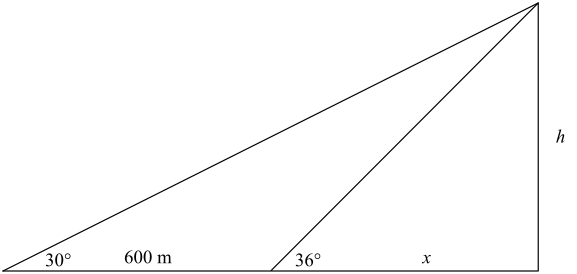
\includegraphics[width=10cm]{L4SZ281I}
\begin{equation*}\frac{h}{x} =\tan  \ang{36} \text{and}\frac{h}{x +600} =\tan  \ang{30} 
\end{equation*}
We want $h$ so we eliminate $x$ between these two equations
\begin{align*}x &  =  \frac{h}{\tan  \ang{36} }\text{and}x +600 =\frac{h}{\tan  \ang{30} } \\
\frac{h}{\tan  \ang{30} } &  =  \frac{h}{\tan  \ang{36} } +600 \\
\frac{h}{\tan  \ang{30} } -\frac{h}{\tan  \ang{36} } &  =  600 \\
h \left (\frac{1}{\tan  \ang{30} } -\frac{1}{\tan  \ang{36} }\right ) &  =  600 \\
h \genfrac{(}{)}{}{}{\tan  \ang{36}  -\tan  \ang{30} }{\tan  \ang{30}  \tan  \ang{36} } &  =  600 \\
h &  =  600 \times \frac{\tan  \ang{30}  \tan  \ang{36} }{\tan  \ang{36}  -\tan  \ang{30} } \\
 &  \approx   600 \times 2.811603815 \\
 &  \approx   1687 \mbox{m}\end{align*}

%---------------------------------------------------
% identities
%---------------------------------------------------
\subsection*{Identities}\label{sec:identities}
The unit circle has equation $x^{2} +y^{2} =1$ and we define $x =\cos  \theta$ and $y =\sin  \theta$ so
\begin{equation*}x^{2} +y^{2} =1 \leadsto \left (\cos  \theta\right )^{2} +\left (\sin  \theta\right )^{2} =1
\end{equation*}
This is always written
\begin{tcolorbox}\[\sin ^{2} \theta +\cos ^{2} \theta =1\]
\end{tcolorbox}
This is an \emph{identity} which means it is true for all values of $\theta$. There are many identities in trigonometry, we will only use the Pythagorean identity (above) and one more.
Given $\sin =\frac{\text{opp}}{\text{adj}}$ we can solve for $\text{opp}=(\sin)(\text{hyp})$. Similarly from cosine:  $\text{adj}=(\cos)(\text{hyp})$. Substituting these into the tangent relationship:
\begin{tcolorbox}\[\tan=\frac{\text{opp}}{\text{adj}}=\frac{(\sin)(\text{hyp})}{(\cos)(\text{hyp})}=\frac{\sin}{\cos}\]
\end{tcolorbox}
The sine and cosine law are two more unique relationships that we will cover in section~\ref{sec:applications}.

%---------------------------------------------------
% trig functions
%---------------------------------------------------
\subsection*{All Students Take Calculus}
In the previous section the angles were between $\ang{0} $ and $\ang{90} $. In this section the angles can take any value. Initially we consider angles between $\ang{0} $ and $\ang{360} $ and relate these to the radian measure between $0$ and $2 \pi $. We remind you that angles are measured anticlockwise from the positive $x$-axis. 

If the point $P (x ,y)$ is in the first quadrant, $\theta $ is the angle between $OP$ and the positive $x$-axis and we complete the right triangle then we have created the following situation.  

\begin {multicols}{2}
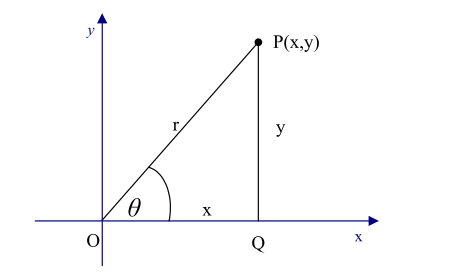
\includegraphics[ width=3.774in, height=2.3454in,]{L4SZ281S}

Let the hypotenuse be $r$ then
\begin{equation*}r =\sqrt{x^{2} +y^{2}}
\end{equation*}
Therefore
\begin{equation*}\sin  \theta  =\frac{y}{r}\text{}\cos  \theta  =\frac{x}{r}\text{and}\tan  \theta  =\frac{y}{x}
\end{equation*}
\end {multicols}
\begin {multicols}{2}
We now let $\theta $ be any angle and define sine, cosine and tangent in the same way. For instance
if $P (x ,y)$ is in the second quadrant:    

$\sin  \theta  =\frac{y}{r}$ because $y$ is positive $\sin  \theta $ will be positive. ($r$ is positive by convention.) 

$\cos  \theta  =\frac{x}{r}$ because $x$ is negative $\cos  \theta $ will be negative. 

$\tan  \theta  =\frac{y}{x}$ because $y$ is positive and $x$ is negative $\tan  \theta $ will be negative. 
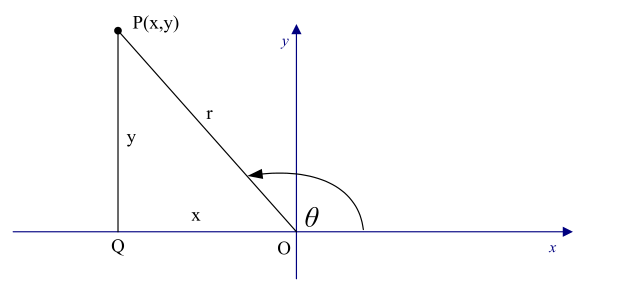
\includegraphics[ width=3.9868in, height=1.8161in,]{L4SZ281T}
\end{multicols}
This pattern can be extended to quadrants 3 and 4. The mnemonic (\textbf{A}ll \textbf{S}tudents \textbf{T}ake \textbf{C}alculus) might help you remember which one is positive although you can always work it out if you need to. 

The value of a trigonometric function consists of two parts the numerical part and the sign. you must get both parts correct. In the previous section you related the values of a terminal point to another point in the first quadrant. A point on the unit circle could be in any one of the four quadrants. 

\qquad \qquad \qquad \qquad
\begin{tabular}[c]{|c|c|c|c|c|c|}\hline
	Quadrant  & $x$-coordinate  & $y$-coordinate  & $\cos $  & $\sin $  & $\tan $  \\
	\hline
	$1$  & $ +$  & $ +$  & $ +$  & $ +$  & $ +$  \\
	\hline
	$2$  & $ -$  & $ +$  & $ -$  & $ +$  & $ -$  \\
	\hline
	$3$  & $ -$  & $ -$  & $ -$  & $ -$  & $ +$  \\
	\hline
	$4$  & $ +$  & $ -$  & $ +$  & $ -$  & $ -$  \\
	\hline
\end{tabular}

Some people learn this as a mnemonic All sin tan cos. (Meaning all are positive in the first quadrant, only sine is positive in the second quadrant, only tangent is positive in the third quadrant and only cosine is positive in the fourth quadrant.) 

\subsection*{The Area of a Triangle}
The fundamental formula for the area of a triangle is $\text{Area} =\frac{1}{2} \times \text{base} \times \text{height}$ Using the trigonometric functions the height can be replaced and the formula becomes:
\begin{equation*}\text{Area} =\frac{1}{2} \times \text{product of two sides} \times \text{sine of the included angle}
\end{equation*}
The formula is particularly easy to remember in symbolic form. Let the triangle have vertices $A$, $B$ and $C$, so the the sides opposite these angles are $a$, $b$ and $c$ respectively. Then the area can be expressed symbolically as
\begin{equation*}\text{Area} =\frac{1}{2} a b \sin  C =\frac{1}{2} b c \sin  A =\frac{1}{2} a c \sin  B
\end{equation*}

\columnsep =30pt
\begin {multicols}{2} 
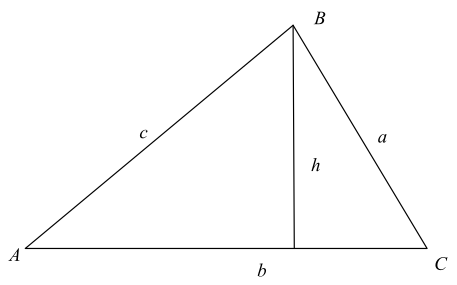
\includegraphics[width=8cm]{L4SZ281U}

\begin{align*}\sin  A &  = \frac{h}{c}\text{ and }h =c \sin  A \\
\text{Area} &  =  \frac{1}{2} \times \text{base} \times \text{height} \\
 &  =  \frac{1}{2} \times b \times c \sin  A =\frac{1}{2} b c \sin  A
 \end{align*}
\end {multicols}
It depends where you draw $h$ and which angle you choose to use as to which formula you finish up with. The key point to remember is $b$ and $c$ are two sides and $A$ is the angle between them. The triangle above shows $A$ as an acute angle (between $\ang{0}$ and $\ang{90} $). If the angle is obtuse (between $\ang{90} $ and $\ang{180} $) the formula still holds. 
\begin{multicols}{2}
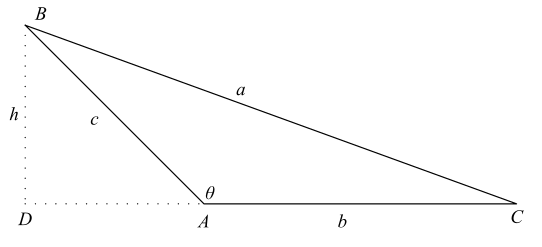
\includegraphics[ width=8cm]{L4SZ281V}
The angle is in the second quadrant and $\sin  (180 -\theta ) =\sin  \theta $, so $\sin  (180 -\theta ) =\frac{h}{c}$ can be written as $\sin  \theta  =\frac{h}{c}$ or $h =c \sin  \theta $ or $h =c \sin  A$ where $A$ is obtuse. So the area is $\frac{1}{2} b c \sin  A$ 
\end{multicols}
\textbf{Example} A triangle has two sides of $5 \mbox{cm}$ and $8 \mbox{cm}$ and the angle between them is $\ang{150} $. Find its area.
\begin{equation*}\text{Area} =\frac{1}{2} \times 5 \times 8 \times \sin  \ang{150} 
\end{equation*}

It helps to remember that $\sin  150 =\sin  30 =\frac{1}{2}$
\begin{equation*}\text{Area} =\frac{1}{2} \times 5 \times 8 \times \frac{1}{2} =10 \text{ cm}^{2}
\end{equation*}

%---------------------------------------------------
% TRIG FUNCTIONS & GRAPHS
%---------------------------------------------------
\section{Trig Functions of Real Numbers}
In this next part of the chapter the three main trigonometric functions (sine, cosine and tangent) will be studied. They will be viewed as functions of real numbers rather than angles. The trigonometric functions defined in these two ways are identical and there is a simple rule connecting the domains. Why do we show you the two approaches? Trigonometry will be used to solve a variety of problems and these can be divided into two groups, dynamic problems and static problems. When dynamic problems (such as problems involving motion) are being solved real numbers will be used. When static problems (such as finding distances and angles for triangles) are being solved angles will be used. 

%---------------------------------------------------
% trig graphs
%---------------------------------------------------
%\section{Trigonometric Functions}
You should be familiar with the fundamental graphs of $y =\sin  x$ and $y =\cos  x$. These graphs are the basis of this section. \Desmos can easily show you the shape of $y =\sin  x$ and $y =\cos  x$ so if you are asked to draw a rough sketch of these curves you should plot a few key points and draw a smooth curve between them. You will usually be given the required domain however if you are not you would choose to draw these for one complete cycle ($0 -2 \pi $). To sketch $y =\sin  x$ it is enough to select as key points $x =0$, $\frac{\pi }{2}$, $\pi $, $\frac{3 \pi }{2}$, $2 \pi $. 


\begin{tabular}[c]{|l|l|l|l|l|l|}\hline
	$x$  & $0$  & $\frac{\pi }{2}$  & $\pi $  & $\frac{3 \pi }{2}$  & $2 \pi $  \\
	\hline
	$y =\sin  x$  & $0$  & $1$  & $0$  & $ -1$  & $0$  \\
	\hline
\end{tabular}

Similarly to sketch $y =\cos x$ the same values of $x$ give 


\begin{tabular}[c]{|l|l|l|l|l|l|}\hline
	$x$  & $0$  & $\frac{\pi }{2}$  & $\pi $  & $\frac{3 \pi }{2}$  & $2 \pi $  \\
	\hline
	$y =\cos  x$  & $1$  & $0$  & $ -1$  & $0$  & $1$  \\
	\hline
\end{tabular}

You will be aware that these curves repeat this pattern every $2 \pi $ where $x$ extends in both the positive and negative directions. 

$0 -2 \pi $ represents one complete cycle. Mathematically we say
\begin{align*}\sin  \left (x +2 n \pi \right ) &  = \sin  x\text{\  for any integer}n \\
	\cos  \left (x +2 n \pi \right ) &  = \cos  x\text{\  for any integer}n\end{align*}

Aside: instead of "for any integer $n$" we can write $ \forall n \in \mathbb{Z}$. 

A function that displays this characteristic is described as \emph{periodic} and for $y =\sin x$ and $y =\cos x$ the \emph{period} is $2 \pi $. 

You will often be asked to state the period of a trigonometric function so for sine and cosine it
is wise to remember that often the period is $2 \pi $. This means you need only worry about the distinctly different class of examples
of sine and cosine where the period is not $2 \pi $. 

You will sometimes be asked to sketch a graph for a given number of periods or a given number of cycles. These are two different ways of saying the same thing. 

\subsection{Transformations}
The following six transformations can be applied to any function including sine, cosine, and tangent. 
\begin{tasks}[style=itemize](3)
\task Vertical shift 
\task Horizontal shift 
\task Vertical stretch 
\task Horizontal stretch 
\task Reflection in the $x$-axis 
\task Reflection in the $y$-axis 
\end{tasks}

\textbf{Example 1}
Sketch $y =\sin  \left (x -\frac{\pi }{2}\right ) +3$ \\
1. This may be considered as a sine curve shifted $\frac{\pi }{2}$ to the right and $3$ upwards.\\ 
\textbf{Definition:} A horizontal shift of a sine curve or cosine curve is called a \emph{phase shift}. \\
2. Transform the 5 point summary \\
\begin{tabular}{llllll}\toprule
	$x$  & $0$  & $\frac{\pi }{2}$  & $\pi $  & $\frac{3 \pi }{2}$  & $2 \pi $  \\
	\midrule
	$\sin  x$  & $0$  & $1$  & $0$  & $ -1$  & $0$  \\
	\midrule
	$\sin  \left (x -\frac{\pi }{2}\right )$  & $ -1$  & $0$  & $1$  & $0$  & $ -1$  \\
	\midrule
	$\sin  \left (x -\frac{\pi }{2}\right ) +3$  & $2$  & $3$  & $4$  & $3$  & $2$  \\
	\bottomrule
\end{tabular}

3. The difference between this approach and the previous one is that the values are calculated
from the 5 values of $x$. Maybe an additional row containing $x -\frac{\pi }{2}$ values will help. \\
\begin{tabular}{llllll}\toprule
	$x$  & $0$  & $\frac{\pi }{2}$  & $\pi $  & $\frac{3 \pi }{2}$  & $2 \pi $  \\
	\midrule
	$x -\frac{\pi }{2}$  & $ -\frac{\pi }{2}$  & $0$  & $\frac{\pi }{2}$  & $\pi $  & $\frac{3 \pi }{2}$  \\
	\midrule
	$\sin  \left (x -\frac{\pi }{2}\right ) +3$  & $2$  & $3$  & $4$  & $3$  & $2$  \\
	\bottomrule
\end{tabular}

4. Desmos confirms this. The plot shows $y=\sin x$ as reference.\\
\begin{center}
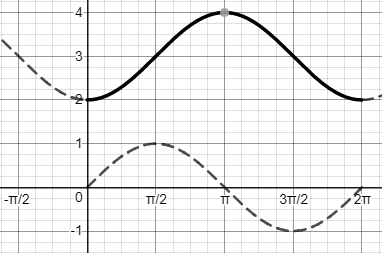
\includegraphics[width=8cm]{trigShift1}
\end{center}


\textbf{Example 2} Sketch $y =\cos  (x -\frac{\pi }{6})$.
\textbf{Solution} You could use a table of values however this is $y =\cos  x$ with a horizontal shift of $\frac{\pi }{6}$ to the right. Sketch the transformation on top of the graph of $y =\cos  x $.
\begin{center}
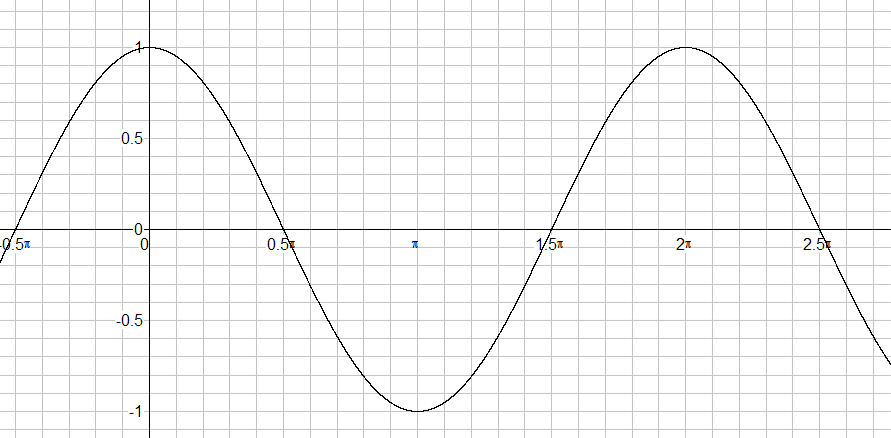
\includegraphics[width=10cm]{L4SZ270H}
\end{center}

In general $y =a \sin  x$ represents a vertical stretch of $y =\sin  x$ by $a$. If $a$ is negative the transformation can either be described as a negative stretch or (preferably) as a \emph{stretch}
of $\left \vert a\right \vert $ followed by a \emph{reflection} in the $x$-axis. Recall the reflection of $y =f \left (x\right )$ in the $x$-axis is $y = -f \left (x\right )$. The number $\left \vert a\right \vert $ is called the \emph{amplitude} for both $y =\sin  x$ and $y =\cos  x\text{.}$ 

If $0 <a <1$ the fractional stretch causes the curve to shrink vertically. For instance the curve
$y =\sin  x$ has a maximum value of $1$ and a minimum value of $ -1$. the curve $y =\frac{1}{2} \sin  x$ has a maximum value of $\frac{1}{2}$ and a minimum value of $ -\frac{1}{2}$. 

\textbf{Example 4} Sketch $y =\cos  ( -t)\text{.}$ 

Recall the reflection of $y =f (x)$in the $y$-axis is $y =f ( -x)$ so you would expect $y =\cos  ( -t)$ to be the reflection of $y =\cos  t$ in the $y$-axis. 


\textbf{Example 5} Sketch $y =\sin \left( \frac{1}{2}x\right)$ 


\textbf{Example 6} Sketch $y =\cos(2x)$ 




\subsection{Tangent}
This section in the textbook covers the tangent, cotangent, secant and cosecant functions. In this course we will concentrate on the tangent function. the remaining three functions (often called the reciprocal functions) will only be covered when they are needed. By focussing on sine, cosine and tangent the majority of problems we encounter can be solved. Furthermore these are the functions we can evaluate immediately by pressing appropriate keys on the calculator. 

Previously we learnt that the period for the sine and cosine functions was $2 \pi $. Tangent is also a periodic function and it has a period of $\pi $ (not $2 \pi $). This means that it goes through one complete cycle every $2 \pi $. Recall $\tan  t =\frac{\sin  t}{\cos  t}$. To analyse the behaviour of the tangent function it helps if you know what you are looking for. You should know the shape of $y =\tan  t$ from previous courses. Some key values of tangent will show the pattern. 


\begin{tabular}[c]{|l|l|l|l|}\hline
	$t$  & $\sin  t$  & $\cos  t$  & $\tan  t$  \\
	\hline
	$ -\frac{\pi }{2}$  & $ -1$  & $0$  & $\frac{ -1}{0} = -\infty $  \\
	\hline
	$ -\frac{\pi }{4}$  & $ -\frac{\sqrt{2}}{2}$  & $\frac{\sqrt{2}}{2}$  & $ -\frac{\sqrt{2}}{2} \div \frac{\sqrt{2}}{2} = -1$  \\
	\hline
	$0$  & $0$  & $1$  & $\frac{0}{1} =0$  \\
	\hline
	$\frac{\pi }{4}$  & $\frac{\sqrt{2}}{2}$  & $\frac{\sqrt{2}}{2}$  & $\frac{\sqrt{2}}{2} \div \frac{\sqrt{2}}{2} =1$  \\
	\hline
	$\frac{\pi }{2}$  & $1$  & $0$  & $\frac{1}{0} =\infty $  \\
	\hline
\end{tabular}

As $t$ takes values from $ -\frac{\pi }{2}$ to $\frac{\pi }{2}$, $\tan  t$ takes values from $ -\infty $ to $\infty $. This pattern is repeated every $\pi $. Mathematically we say
\begin{equation*}\tan  \left (t +n \pi \right ) =\tan  t\text{\  } \forall n \in \mathbb{Z}
\end{equation*}

Furthermore $y =\tan  t$ is an \emph{odd function} so
\begin{equation*}\tan  \left ( -t\right ) = -\tan  t
\end{equation*}

A Desmos graph can show this relationship 

\setlength\fboxrule{0.01in}\setlength\fboxsep{0.2in}\fcolorbox[HTML]{000000}{FFFFFF}{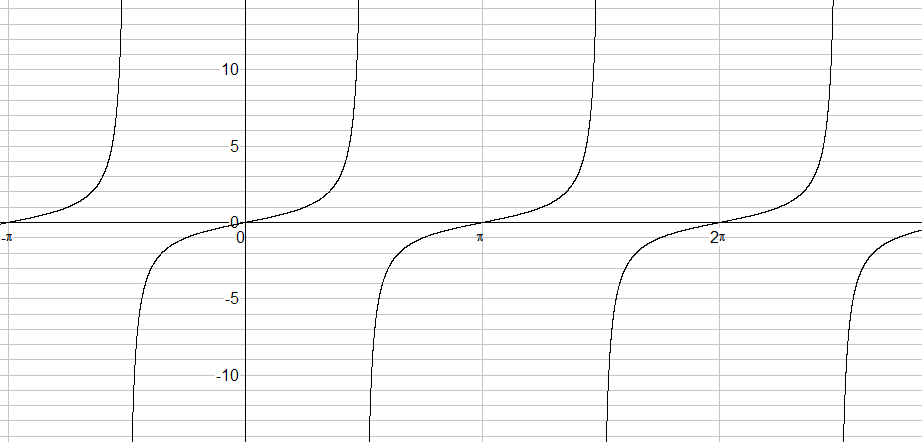
\includegraphics[ width=5.9646in, height=2.8772in,]{L4SZ270M}}

The graph can be seen to have point symmetry. If you rotate the tangent curve through a half turn using the origin as axis the curve will lie on top of itself. This is a pictorial representation of an odd function.

Aside: You must not confuse $y =\tan  x$ with $y =x^{3}$. While they may appear to be similar in shape the only similarities are that they both pass through the origin and continue towards $\infty $ in the first quadrant and $ -\infty $ in the third quadrant. Important differences that you should identify if you are asked to sketch these graphs are the slope of the curves at the origin and the behaviour as $y \leadsto  \pm \infty $. 

%---------------------------------------------------
% sine rule and cosing rule
%---------------------------------------------------
\section{Applications}\label{sec:applications}
\subsection{The Sine Rule}
In this section we use the Sine Rule to find the sides and angles in triangles without a right angle. In the next section we use the Cosine Rule to find sides and angles in triangles also, so as you study these two sections you need to learn which problems require the Sine Rule and which require the Cosine Rule. 

Previously, we met the formula for the area of a triangle. given two sides and the included angle $\left ( =\frac{1}{2} a b \sin  C\right )$. The Sine Rule and Cosine Rule also require specific combinations of sides and angles. 

The easiest way to visualise the situations in which the two rules are used is to use the labelling we met in section $3.3$. Let the triangle be $ \Delta A B C$ and let the sides be $a$, $b$ and $c$ where $a$ is opposite $\angle A$ etc. 

\setlength\fboxrule{0in}\setlength\fboxsep{0.2in}\fcolorbox[HTML]{000000}{FFFFFF}{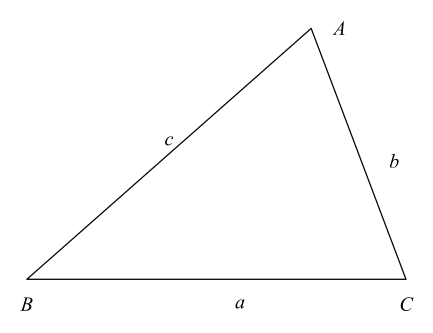
\includegraphics[ width=3.1358in, height=2.4171in,]{L4SZ281W}}

\begin{tabular}[c]{lll}\textbf{Sine Rule}  &  & \textbf{Cosine
		Rule}  \\
	Given a side and the angle opposite the side  &  & \textbf{(a)}
	Given two sides and the included angle  \\
	\textbf{(a)} If a second angle is
	given the Sine Rule  &  & the Cosine Rule allows us to find the
	side  \\
	allows us the side opposite that angle  &  & opposite
	the angle  \\
	Given $A$, $a$ and $B$ use the Sine Rule to find $b\text{.}$  &  & Given $a$, $b$ and $C$ use the Cosine Rule to find $c\text{.}$  \\
	\textbf{(b)} If a second
	angle is given and the side that  &  & \textbf{(b)} Given three
	sides the Cosine Rule allows  \\
	is not opposite that angle is required then first  &  & us
	to find any angle.  \\
	find the third angle then use (a).  &  & Given
	$a$, $b$ and $c$ use the Cosine Rule to find $A$  \\
	Given $A$, $a$ and $B$ where $c$ is required  &  & or $B$ or $C$.  \\
	1. $C =180 -(A +B)$  &  &  \\
	2.
	Use the Sine Rule to find $c$.  &  &  \\
	\textbf{(c)} If a second side is given the Sine Rule  &  &  \\
	allows
	us to find the angle opposite that side.  &  &  \\
	Given
	$A$, $a$, and $b$ use the Sine Rule to find $B$.  &  &  \\
\end{tabular}

Textbooks may use the term ``The Law of Sines" whereas in these notes the term ``The Sine Rule will be used. 

\begin{tcolorbox}
	The Sine Rule states that in any triangle
	\begin{equation*}\frac{\sin  A}{a} =\frac{\sin  B}{b} =\frac{\sin  C}{c}
	\end{equation*}\end{tcolorbox}
This can also be written inversely:
\begin{equation*}\frac{a}{\sin  A} =\frac{b}{\sin  B} =\frac{c}{\sin  C}
\end{equation*}

\subsection*{Proof of the Sine Rule}
The Sine Rule is easy to prove from the formula for the area of a triangle
\begin{equation*}\text{Area} =\frac{1}{2} b c \sin  A =\frac{1}{2} a c \sin  B =\frac{1}{2} a b \sin  C
\end{equation*}

Multiply right through by 2
\begin{equation*}b c \sin  A =a c \sin  B =a b \sin  C
\end{equation*}

Divide right through by $a b c$
\begin{equation*}\frac{\sin  A}{a} =\frac{\sin  B}{b} =\frac{\sin  C}{c}
\end{equation*}

Fractions can always be inverted as long as the same process is applied to each fraction.
\begin{equation*}\frac{a}{\sin  A} =\frac{b}{\sin  B} =\frac{c}{\sin  C}
\end{equation*}

\textbf{Example 1} Find side lengths $a$ and $c$ in the following triangle.

\setlength\fboxrule{0in}\setlength\fboxsep{0.2in}\fcolorbox[HTML]{000000}{FFFFFF}{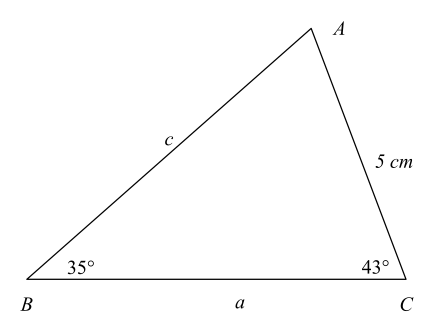
\includegraphics[ width=2.6143in, height=2.0159in,]{L4SZ281X}
}
\\\relax (a) To find $c$
\begin{align*}\frac{c}{\sin  C} &  = \frac{b}{\sin  B} \\
\frac{c}{\sin  43 } &  = \frac{5}{\sin  35 } \\
c &  = \frac{5 \sin  43 }{\sin  35 } \\
&  \approx   5.945139277 \approx 5.9 \mbox{cm}\text{(1 dp)}\end{align*} \\\relax (b) To find $a$ 

(i) $A =\ang{180}  -(\ang{35}  +\ang{43} ) =\ang{180}  -\ang{78}  =\ang{102} $ 

(ii) It is usually wise to go back to the original data (i.e. use $b$ and $B$ rather than $c$ and $C$).
\begin{align*}\frac{a}{\sin  A} &  = \frac{b}{\sin  B} \\
\frac{a}{\sin  102 } &  = \frac{5}{\sin  35 } \\
a &  = \frac{5 \sin  102 }{\sin  35 } \\
&  \approx   8.526741501 \approx 8.5 \mbox{cm}\text{(1 dp)}\end{align*}

These two calculations illustrate the first two cases in which the Sine Rule is used. You will notice that the triangle has been completely solved in the course of this example. We started with one side and two angles and we found the other two sides and the other angle. 

The third case is not as straight forward. Given two sides and an angle there could be no triangle formed, one triangle formed or two triangles formed depending on the length of the side opposite the given angle. You should develop an insight into the reasons why this is so. Imagine the second side given is the boom of a crane and the angle given is the angle between the boom and the ground. The side opposite the given angle is represented by the cable. It is clear that for certain lengths of the cable the hook will not reach the ground. Then as the hook is lowered a point will be reached when the hook just touches the ground.  

\columnsep =30pt
\begin {multicols}{2}
\setlength\fboxrule{0in}\setlength\fboxsep{0.2in}\fcolorbox[HTML]{000000}{FFFFFF}{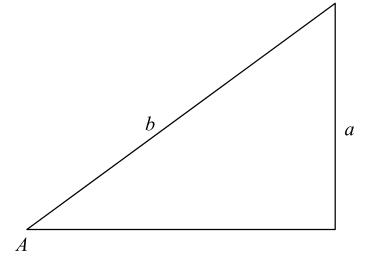
\includegraphics[ width=2.9577in, height=2.2061in,]{L4SZ281Y}}

It is no surprise that the length $a$ to create this situation is $a =b \sin  A\text{.}$ 

We are after all dealing with the Sine Rule which becomes the fundamental sine formula $\left (\sin  A =\frac{\text{opp}}{\text{hyp}} =\frac{a}{b}\right )$ when the triangle has a right angle. 
\end {multicols}

If the cable is held taut and is extended a little more it will touch the ground in two places (provided it is kept in the same plane). As the cable is extended further the time will come where the cable is as long as boom. At this point there is only one solution again, the one straight out in front of the crane). Further extensions of the cable will produce only one solution (straight out in front of the crane) as the cable will theoretically reach behind the crane boom thus creating a different triangle altogether. 

The two solutions case is often referred to as the ambiguous case. The discussion above shows the range of values of $a$ that will give two solutions.
\begin{equation*}b \sin  A <a <b
\end{equation*}

\textbf{Example 2} Given $a =\ang{30} $, $a =8$ and $b =7$ solve the triangle (i.e. find $B$, $C$ and $c$).    
\setlength\fboxrule{0in}\setlength\fboxsep{0.2in}\fcolorbox[HTML]{000000}{FFFFFF}{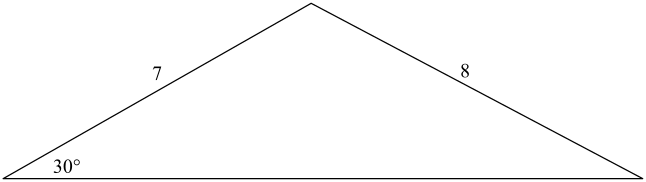
\includegraphics[ width=4.2739in, height=1.2202in,]{L4SZ281Z}}

Because $8 >7$ this is the one solution case. 

1. Find $B$
\begin{align*}\frac{\sin  B}{b} &  = \frac{\sin  A}{a} \\
\sin  B &  = \frac{b \sin  A}{a} \\
&  = \frac{7 \sin  30 }{8} =0.4375 \\
B &  = \sin ^{ -1} 0.4375 \approx \ang{25.94} \end{align*}

2. Find $C$
\begin{align*}C &  = \ang{180}  -(\ang{30}  +\ang{25.94} ) \\
&  = \ang{124.06} \end{align*}

3. Find $c$
\begin{align*}\frac{c}{\sin  C} &  = \frac{a}{\sin  A} \\
c &  = \frac{a \sin  C}{\sin a} \\
&  = \frac{8 \sin  124.06 }{\sin  30 } \\
&  \approx   13.3\end{align*}

%--------ambiguous case example---------------------------
\textbf{Example 3 - The Ambiguous Case} Given $A =\ang{30} $, $a =6$ and $b =7$ solve the triangle. 

In this case $b \sin  A =3.5$ and $b =7$ so as $a$ lies between $3.5$ and $7$. This is the ambiguous case, therefore there are two solutions. 
\columnsep =30pt
\begin {multicols}{2}
\setlength\fboxrule{0in}\setlength\fboxsep{0.2in}\fcolorbox[HTML]{000000}{FFFFFF}{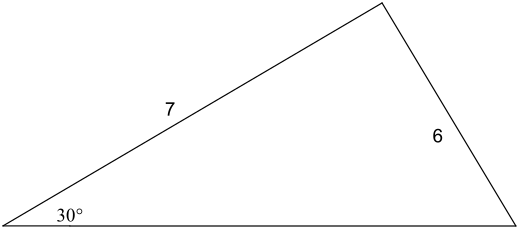
\includegraphics[ width=2.8885in, height=1.2825in,]{L4SZ2820}}

\setlength\fboxrule{0in}\setlength\fboxsep{0.2in}\fcolorbox[HTML]{000000}{FFFFFF}{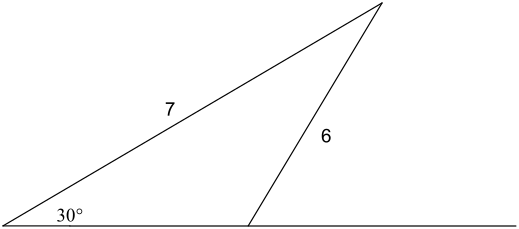
\includegraphics[ width=2.9308in, height=1.3015in,]{L4SZ2821}}
\end {multicols}
It is best to visualise these two solutions on the same diagram so that the isosceles triangle can help lead to the two results. 

\setlength\fboxrule{0in}\setlength\fboxsep{0.2in}\fcolorbox[HTML]{000000}{FFFFFF}{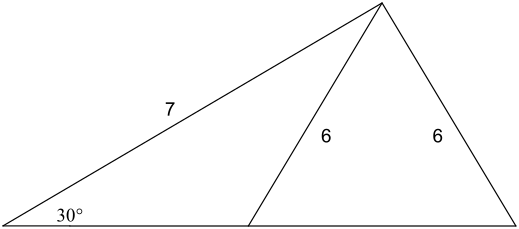
\includegraphics[ width=2.9585in, height=1.3136in,]{L4SZ2822}}

\textbf{First solution} (Proceed as before) 
1. Find $B$
\begin{align*}\frac{\sin  B}{b} &  = \frac{\sin  A}{a} \\
\sin  B &  = \frac{b \sin  A}{a} \\
&  = \frac{7 \sin  30 }{6} =0.58 \dot{3} \\
B &  = \sin ^{ -1} 0.58 \dot{3} \approx \ang{35.69} \end{align*}

2. Find $C$
\begin{align*}C &  = \ang{180}  -(\ang{30}  +\ang{35.69} ) \\
&  = \ang{114.31} \end{align*}

3. Find $c$
\begin{align*}\frac{c}{\sin  C} &  = \frac{a}{\sin  A} \\
c &  = \frac{a \sin  C}{\sin  A} \\
&  = \frac{6 \sin  114.31 }{\sin  30 } \\
&  \approx   10.9\end{align*}

\textbf{Second solution} 
1. Find the second value of $B$ 

\begin{equation*}B =\ang{180}  -\ang{35.69}  =\ang{144.31} 
\end{equation*}

2. Find $C$
\begin{equation*}C =\ang{180} -(\ang{30}  +\ang{144.31} ) =\ang{180}  -\ang{174.31}  =\ang{5.69} 
\end{equation*}

(Or if you remember the rule that the exterior angle of a triangle is the sum of the two interior
opposite angles $C +\ang{30}  =\ang{35.69} $ so $C =\ang{35.69}  -\ang{30}  =\ang{5.69} $) 

3. Find $c$
\begin{align*}\frac{c}{\sin  C} &  = \frac{a}{\sin  A} \\
c &  = \frac{a \sin  C}{\sin  A} \\
&  = \frac{6 \sin  5.69 }{\sin  30 } \\
&  \approx   1.2\end{align*}

\subsection{The Cosine Rule}
In this section we will state and prove the Cosine Rule (which is called "The Law of Cosines" in the textbook). The proof is given here for completeness. You will not be tested on your ability to reproduce it. The section will give examples where the Cosine Rule is used to solve problems using the \emph{triangle of vectors} and we will include revision of \emph{bearings} and the use of trigonometry in \emph{navigation}. 

\begin{tcolorbox}
	For any triangle side sides $a$, $b$, and $c$ and angle $A$ opposite side $a$:\\
	\begin{center}
		$a^{2} =b^{2} +c^{2} -2 b c \cos  A$
	\end{center}	
\end{tcolorbox}

\subsection*{Proof of The Cosine Rule}
\textbf{To prove:} For any triangle $ \Delta A B C\text{,}$ $a^{2} =b^{2} +c^{2} -2 b c \cos  A$ \\ 
\columnsep =30pt
\begin {multicols}{2}
\setlength\fboxrule{0in}\setlength\fboxsep{0.2in}\fcolorbox[HTML]{000000}{FFFFFF}{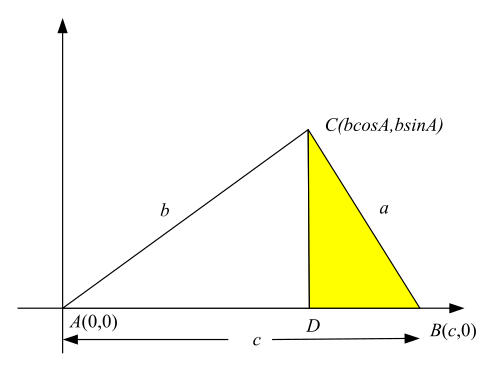
\includegraphics[ width=3.1021in, height=2.3549in,]{L4SZ282A}}
By Pythagoras' Theorem
\begin{align*}B C^{2} &  = C D^{2} +D B^{2} \\
a^{2} &  = \left (c -b \cos  A\right )^{2} +\left (b \sin  A\right )^{2} \\
&  = c^{2} -2 b c \cos  A +b^{2} \cos ^{2} A +b^{2} \sin ^{2} A \\
&  = c^{2} -2 b c \cos  A +b^{2} \left (\cos ^{2} A +\sin ^{2} A\right ) \\
&  = c^{2} -2 b c \cos  A +b^{2}\text{as}\cos ^{2} A +\sin ^{2} A =1\text{\ }\end{align*} 
\end {multicols}
This is usually written
\begin{equation*}a^{2} =b^{2} +c^{2} -2 b c \cos  A
\end{equation*}

The diagram has been drawn to simplify the way the proof unfolds. You will see that by placing the vertex $A$ at the origin the side $a$ is found in terms of $b$, $c$, and $A$. The proof would have been the same had $A$ and $B$ been as shown and $C$ placed in the second quadrant. (Thus producing a triangle with an obtuse angle at $A$.) This rule is symmetrical. You need to be given two sides and the included angle ($b$, $c$ and $A$) and the formula allows you to calculate $a$. Most textbooks will therefore show you three equivalent formulae
\begin{align*}a^{2} &  = b^{2} +c^{2} -2 b c \cos  A \\
b^{2} &  = c^{2} +a^{2} -2 c a \cos  B \\
c^{2} &  = a^{2} +b^{2} -2 a b \cos  C\end{align*}

In this course you will only be given one formula and you will have to know what sides and angles to assign to the variables. 

\textbf{Example 1}
Given $a =5$, $b =6$ and $C =\ang{50} $, find $c$.
\begin{align*}c^{2} &  = a^{2} +b^{2} -2 a b \cos  C \\
&  = 5^{2} +6^{2} -2 \times 5 \times 6 \times \cos  50  \\
&  \approx   22.43274342 \\
c &  \approx   \sqrt{22.43274342} \\
&  \approx   4.736321718 \approx 4.7 \left (1\text{dp}\right )\end{align*}

\textbf{Example 2}
Given $a =5$, $b =6$ and $C =\ang{130} $, find $c$.
\begin{align*}c^{2} &  = a^{2} +b^{2} -2 a b \cos  C \\
&  = 5^{2} +6^{2} -2 \times 5 \times 6 \times \cos  130  \\
&  \approx   99.56725658 \\
c &  \approx   \sqrt{99.56725658} \\
&  \approx   9.97833937 \approx 10.0 \left (1\text{dp}\right )\end{align*}

These two examples show that when the two sides and the included angle are given the third side
(opposite the given angle) can be found. 

\textbf{Example 3} Find the angle given three side lengths; given $a =5$, $b =6$ and $c =9$, find $A$. 

Because $a$ is the smallest side $A$ will most certainly be an acute angle.
\begin{align*}\cos  A &  = \frac{b^{2} +c^{2} -a^{2}}{2 b c} \\
&  = \frac{6^{2} +9^{2} -5^{2}}{2 \times 6 \times 9} \\
&  \approx 0.851851851 \\
A &  \approx \cos ^{ -1} \left (0.851851851\right ) \\
&  \approx \ang{31.6} 
\end{align*}

%---------------------------------------------------
% Chapter Exercises in a separate file
%---------------------------------------------------
\section{Chapter Exercises}
\subimport{}{TrigExercises}

